\documentclass[review]{elsarticle}
\usepackage{subfig}
\usepackage{float} %Permite manejar/mover/partir mejor figuras y tablas
\usepackage{lineno,hyperref}
\usepackage[none]{hyphenat}
\usepackage{eurosym}
\modulolinenumbers[5]

\journal{}

%%%%%%%%%%%%%%%%%%%%%%%
%% Elsevier bibliography styles
%%%%%%%%%%%%%%%%%%%%%%%
%% To change the style, put a % in front of the second line of the current style and
%% remove the % from the second line of the style you would like to use.
%%%%%%%%%%%%%%%%%%%%%%%

%% Numbered
%\bibliographystyle{model1-num-names}

%% Numbered without titles
%\bibliographystyle{model1a-num-names}

%% Harvard
%\bibliographystyle{model2-names.bst}\biboptions{authoryear}

%% Vancouver numbered
%\usepackage{numcompress}\bibliographystyle{model3-num-names}

%% Vancouver name/year
%\usepackage{numcompress}\bibliographystyle{model4-names}\biboptions{authoryear}

%% APA style
%\bibliographystyle{model5-names}\biboptions{authoryear}

%% AMA style
%\usepackage{numcompress}\bibliographystyle{model6-num-names}

%% `Elsevier LaTeX' style
\bibliographystyle{elsarticle-num}
%%%%%%%%%%%%%%%%%%%%%%%

\begin{document}

\begin{frontmatter}

\title{Investigation of the CRT performance of a PET scanner based in liquid xenon: A Monte Carlo study}

%PETALO, a positron emission time-of-flight apparatus using liquid xenon
%\tnotetext[mytitlenote]{Fully documented templates are available in the elsarticle package on \href{http://www.ctan.org/tex-archive/macros/latex/contrib/elsarticle}{CTAN}.}

%% Group authors per affiliation:
\author{J.J. Gomez-Cadenas, J.M. Benlloch-Rodriguez and Paola Ferrario}
\address{IFIC (U. Valencia/CSIC)}
%\fntext[myfootnote]{Since 1880.}

%% or include affiliations in footnotes:
%\author[mymainaddress,mysecondaryaddress]{Elsevier Inc}
%\ead[url]{www.elsevier.com}
%
%\author[mysecondaryaddress]{Global Customer Service\corref{mycorrespondingauthor}}
%\cortext[mycorrespondingauthor]{Corresponding author}
%\ead{support@elsevier.com}
%
%\address[mymainaddress]{1600 John F Kennedy Boulevard, Philadelphia}
%\address[mysecondaryaddress]{360 Park Avenue South, New York}

\begin{abstract}
The measurement of the time of flight of the two 511 keV gammas recorded in coincidence in a PET scanner provides an effective way of reducing the random background and therefore increase the scanner sensitivity, provided that the coincidence resolution time (CRT) of the gammas is sufficiently good. Existing commercial systems based in LYSO crystals, such as the GEMINIS of Philips, reach CRT values of 
$\sim 600$~ps (FWHM). The CRT attained in small setups, however, is much better (around 100-200 ps, depending on the experimental conditions). 

PETALO (Positron Electron TOF Apparatus using Liquid xenOn) is a proposed new type of PET scanner using liquid xenon. The detector building block is the liquid xenon scintillating cell. The cell shape and dimensions can be optimised depending on the intended application. In particular, we consider a box in which two faces are covered by silicon photomultipliers and the others by a reflecting material such as Teflon. The SiPMs can be VUV sensitive or, alternatively, be coated with a wavelength shifter such as tetraphenyl butadiene. The good energy and position resolution of the liquid xenon scintillating cell coupled with the relatively low cost of xenon (a factor 7-8 less than LYSO per unit of detection) and the possibility of relatively sparse instrumentation (e.g, the use of 6 mm SiPMs reducing the number of sensors and electronic channels) makes PETALO suitable for the construction of a large scanner (e.g, full body PET) of high sensitivity.   

In this paper we present a Monte Carlo investigation of the CRT performance of a
PETALO scanner based in a liquid xenon detection cell with two instrumented faces. We show that a CRT of 80 ps FWHM can be achieved if the cell is instrumented with VUV-sensitive SiPMs and a CRT of 100 ps is achieved using blue-sensitive SiPMs coated with TPB. This results show the excellent time of flight capabilities of a PETALO scanner.   
 \end{abstract}

\begin{keyword}
PET \sep TOF \sep liquid xenon \sep energy resolution \sep
 high sensitivity \sep coincidence resolution time (CRT) \sep SiPMs \sep LYSO.
\end{keyword}

\end{frontmatter}

%\linenumbers
% BB
\newcommand{\bb}{\ensuremath{\beta\beta}}
% BB0NU
\newcommand{\bbonu}{\ensuremath{\beta\beta0\nu}}
% BB2NU
\newcommand{\bbtnu}{\ensuremath{\beta\beta2\nu}}
% NME
\newcommand{\Monu}{\ensuremath{\Big|M_{0\nu}\Big|}}
\newcommand{\Mtnu}{\ensuremath{\Big|M_{2\nu}\Big|}}
% PHASE-SPACE FACTOR
\newcommand{\Gonu}{\ensuremath{G_{0\nu}(\Qbb, Z)}}
\newcommand{\Gtnu}{\ensuremath{G_{2\nu}(\Qbb, Z)}}

% mbb
\newcommand{\mbb}{\ensuremath{m_{\beta\beta}}}
\newcommand{\kgy}{\ensuremath{\rm kg \cdot y}}
\newcommand{\ckky}{\ensuremath{\rm counts/(keV \cdot kg \cdot yr)}}
\newcommand{\mbba}{\ensuremath{m_{\beta\beta}^a}}
\newcommand{\mbbb}{\ensuremath{m_{\beta\beta}^b}}
\newcommand{\mbbt}{\ensuremath{m_{\beta\beta}^t}}
\newcommand{\nbb}{\ensuremath{N_{\beta\beta^{0\nu}}}}

% Qbb
\newcommand{\Qbb}{\ensuremath{Q_{\beta\beta}}}

% Tonu
\newcommand{\Tonu}{\ensuremath{T_{1/2}^{0\nu}}}

% Tonu
\newcommand{\Ttnu}{\ensuremath{T_{1/2}^{2\nu}}}

% Xe-136
\newcommand{\Xe}{\ensuremath{^{136}}Xe}
\newcommand{\COT}{\ensuremath{CO_2}}
\newcommand{\CHF}{\ensuremath{CH_4}}
\newcommand{\CFF}{\ensuremath{CF_4}}

% 2S
\newcommand{\TwoS}{\ensuremath{^{2}S_{1/2}}}

\newcommand{\TwoP}{\ensuremath{^{2}P_{1/2}}}

\newcommand{\TwoD}{\ensuremath{^{2}D_{3/2}}}


% Xe-136
\newcommand{\CS}{\ensuremath{^{137}}Cs}

% Xe-136
\newcommand{\NA}{\ensuremath{^{22}}Na}


% Bi-214
\newcommand{\Bi}{\ensuremath{^{214}}Bi}

% Tl-208
\newcommand{\Tl}{\ensuremath{^{208}}Tl}

% Pb-208
\newcommand{\Pb}{\ensuremath{^{208}}Pb}
% Pb-208
\newcommand{\PBD}{\ensuremath{^{210}}Pb}

% Po-214
\newcommand{\Po}{\ensuremath{^{214}}Po}
\newcommand{\Kr}{\ensuremath{^{83}}Kr}

% bru
\newcommand{\bru}{cts/(keV$\cdot$kg$\cdot$y)}
\newcommand{\dten}{10 mm/$\sqrt{\rm m}$}
\newcommand{\dtwo}{2 mm/$\sqrt{\rm m}$}
\newcommand{\BAPP}{\ensuremath{Ba^{++}}}
\newcommand{\BAP}{\ensuremath{Ba^{+}}}

\newcommand{\HPXE}{\sc{HPXe}\rm}
\newcommand{\BATA}{\sc{BaTa}\rm}

% Saltos de carro en tablas
\newcommand{\minitab}[2][l]{\begin{tabular}{#1}#2\end{tabular}}

\newcommand{\thedraft}{0.1.1}% version for referees

\newcommand{\MO}{\ensuremath{{}^{100}{\rm Mo}}}
\newcommand{\SE}{\ensuremath{{}^{82}{\rm Se}}}
\newcommand{\ZR}{\ensuremath{{}^{96}{\rm Zr}}}
\newcommand{\KR}{\ensuremath{{}^{82}{\rm Kr}}}
\newcommand{\ND}{\ensuremath{{}^{150}{\rm Nd}}}
\newcommand{\XE}{\ensuremath{{}^{136}\rm Xe}}
\newcommand{\GE}{\ensuremath{{}^{76}\rm Ge}}
\newcommand{\GES}{\ensuremath{{}^{68}\rm Ge}}
\newcommand{\TE}{\ensuremath{{}^{128}\rm Te}}
\newcommand{\TEX}{\ensuremath{{}^{130}\rm Te}}
\newcommand{\TL}{\ensuremath{{}^{208}\rm{Tl}}}
\newcommand{\CA}{\ensuremath{{}^{48}\rm Ca}}
\newcommand{\CO}{\ensuremath{{}^{60}\rm Co}}
\newcommand{\PO}{\ensuremath{{}^{214\rm Po}}}
\newcommand{\U}{\ensuremath{{}^{235}\rm U}}
\newcommand{\CT}{\ensuremath{{}^{10}\rm C}}
\newcommand{\BE}{\ensuremath{{}^{11}\rm Be}}
\newcommand{\BO}{\ensuremath{{}^{8}\rm Be}}
\newcommand{\UDTO}{\ensuremath{{}^{238}\rm U}}
\newcommand{\CD}{\ensuremath{^{116}{\rm Cd}}}
\newcommand{\THO}{\ensuremath{{}^{232}{\rm Th}}}
\newcommand{\BI}{\ensuremath{{}^{214}}Bi}
\newcommand{\FDG}{\ensuremath{^{18}}F}


\section{Introduction}

PETALO (Positron Electron TOF Apparatus using Liquid xenOn) is a proposed new type of PET scanner using liquid xenon (LXe) \cite{Petalo2015}. The detector building block is the liquid xenon scintillating cell (LXSC). The cell shape and dimensions can be optimised depending on the intended application. In particular the LXSC2 is a box in which two faces are covered by silicon photomultipliers and the others by a reflecting material such as Teflon. The SiPMs can be VUV sensitive or, alternatively, be coated with a wavelength shifter such as tetraphenyl butadiene (TPB).  They are read out by ASICs optimized for excellent timing resolution. PETALO is a compact, homogenous and highly efficient detector which shares many of the desirable properties of monolithic crystals, with the added advantage of high yield and fast scintillation offered by liquid xenon, low noise due to cryogenic operations which virtually eliminates the SiPMs dark current and the potential of low cost. 

The energy and spatial resolution of a PETALO scanner based in LXSC2 cells equipped with 6 mm SiPMs coated with TPB was investigated in \cite{Petalo2015}. The expected energy resolution was found to be 12 \% FWHM (dominated by intrinsic fluctuations in xenon). The expected spatial resolution in the three coordinates is 2 mm FWHM. These results are  comparable to those achieved by monolithic LYSO crystals using a much finer segmentation 
(see, for example, ref.~\cite{VanDamm2011}). 

 \begin{figure}[!bthp]
	\centering
	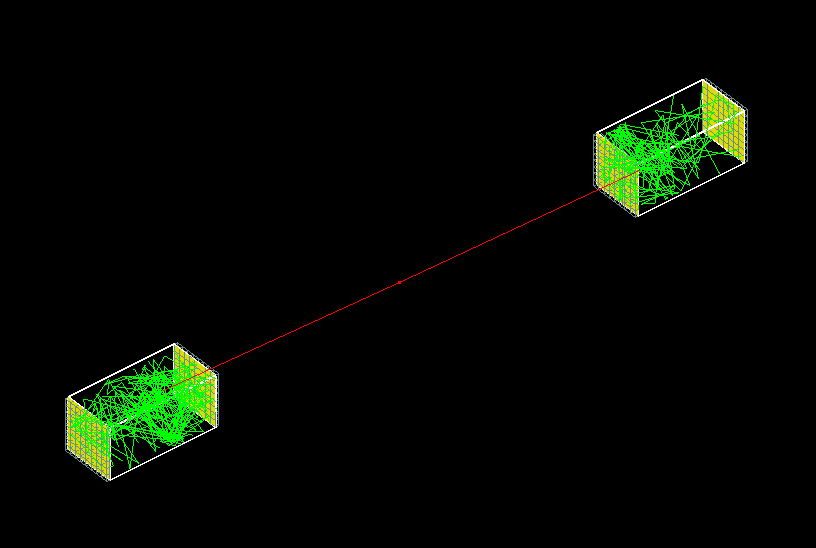
\includegraphics[scale=0.4]{../img/PetaloSetup.png}
	\caption{\label{fig.psetup} Monte Carlo simulation of gamma interactions in the LXe setup, as 
	described in the text.}
\end{figure}

In this paper we present a Monte Carlo investigation of the time resolution
that could be achieved by a PETALO-LXSC2 scanner. To systematically study the different factors that enter the CRT, we have simulated a LXe setup and a LYSO setup, used as a reference. The LXe setup consists of two LXSC2 cells of 
$5 \times 5 \times 5 {\rm ~cm^3}$, facing each other in opposite sides of a 511 keV gamma source 
(Figure \ref{fig.psetup}) and equipped with SiPMs which can be either VUV sensitive or coated with  TPB. The  LYSO setup replaces the two LXSC2 cells by a pair of  monolithic LYSO crystals, also readout by SiPMs, of identical transverse dimensions ($5 \times 5 {\rm ~cm^2}$) and identical thickness in terms of interaction lengths ($1.7 {\rm cm}$).  

This work is organized as follows. In section \ref{sec.LXe} we summarize the relevant properties of liquid xenon as scintillating material and briefly describe the PETALO concept and the expected performance of the LXSC2 in energy and spatial resolution. In section \ref{sec.scint} we review the mechanisms which produce scintillation light in LXe and propose a parameterization of the measured scintillation data in terms of two decay constants. In section \ref{sec.CRT} we discuss the the CRT performance of the LXSC2. Conclusions are presented in section \ref{sec.conclu}. 

\section{Liquid xenon as detection material and the PETALO concept}
\label{sec.LXe}

Xenon is a noble gas. It responds to the interaction of ionizing radiation providing about 60 VUV photons (average wavelength of 178 nm) per keV of deposited energy. The scintillation signal is fast 
(see section \ref{sec.scint}) and can thus result in an excellent CRT.  In its liquid phase (at a temperature of 165 K and atmospheric pressure) LXe has a reasonable high density (3 g/cm$^3$) and an acceptable attenuation length (36 mm), which makes it suitable for PET applications. Its main attractive features are:

\begin{enumerate}
\item {\bf A high scintillation yield (30,000 photons per 511 keV gamma)}, twice as large as that of LYSO. 
\item {\bf LXe is a continuous medium with uniform response}. The design of a compact system is much simpler, then, than when using solid detectors of fixed shape. It is also possible to provide a 3D measurement of the interaction point, and, thus, a high resolution measurement of the DOI. Furthermore, in LXe it is possible to identify Compton events depositing all its energy in the detector as separate-site interaction, due to its relatively large interaction length. This increases the sensitivity of the system, since those events can, in principle, be used for image reconstruction. 
\item {\bf The temperature of LXe at atmospheric pressure (160 K or -113 C)} is hot enough as to permit a simple cryostat, as well as normal operation of the SiPMs, but cold enough to reduce the dark current rate (DCR) of the SiPMs by a factor $\sim 2^{13}$, thus making it essentially negligible. 
\item {The cost} of LXe is 3 \$/cc to be compared with $\sim$ 40-50 \$/cc in the case of LYSO. 
 \end{enumerate}

The first idea of using a LXe time projection chamber for PET was proposed in 1993 by Chepel\cite{chepelFirst}. 
The possibility of building a LXe PET based on the excellent properties of LXe as scintillator, was first suggested by Lavoie in 1976 \cite{lavoie}, and the study of this type of PET was carried out by the Waseda group \cite{Doke1,Nishikido2,Nishikido1}. The Waseda prototype was based in LXe cells read out by VUV-sensitive PMTs which covered 5 of the 6 sides of the cell. 

\begin{figure}[!htbp]
	\centering
	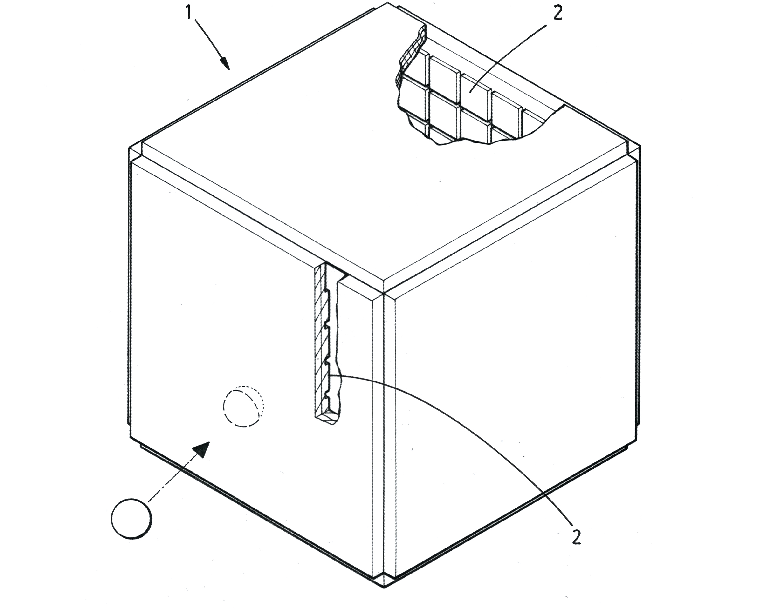
\includegraphics[scale=0.6]{../img/LXSC2.pdf}
	\caption{\label{fig.box} The LXSC2 instruments the entry and exit faces of the box (relative to the photon line of flight) with silicon photomultipliers (SiPMs), which can be eventually coated with TPB. The non-instrumented faces are covered by reflecting Teflon (optionally also coated with TPB). The typical size of the LXSC2
	is $5 \times 5 \times 5 {\rm ~cm^3}$.}
\end{figure}

In the PETALO concept, the PMT-cell is replaced by the Liquid Xenon Scintillating Cell. In particular, the LXSC2 
(Fig.~\ref{fig.box}) instruments the entry and exit faces of the box (relative to the photon line of flight) with silicon photomultipliers (SiPMs), which can be eventually coated with TPB. The non-instrumented faces are covered by reflecting Teflon (optionally also coated with TPB). The shape and the size of the LXSC can be adapted to the application, for example:
\begin{itemize}
\item A scanner designed for large axial coverage (e.g, ``full body PET'') could be based on trapezoidal cells (to maximize the packing) of large transverse dimensions and a thickness of 5 cm (to stop $\sim$80\% of the incoming gammas). To minimize costs, the cell could be instrumented with large
SiPMs (e.g., 6 mm length) coated with TPB.  Note that TPB shifts the VUV light emitted by the LXe  to wavelengths around 430 nm (where the PDE of conventional SiPMs is maximal) with an efficiency of 
80\%. Furthermore, TPB does not absorb blue light above 400 nm, therefore minimizing losses. On the other hand, several manufacturers offer today SiPMs of large area, high gain, low dark current and very low noise which can operate at liquid xenon temperatures with excellent performance.
\item A scanner designed to maximize the sensitivity (with applications, for example
to brain studies) could be based in LXSC2 instrumented with VUV-sensitive SiPMs to optimize the CRT. 
\end{itemize}

The energy resolution R of a liquid xenon scintillation detector is a combination of light collection variation due to the detector geometry R$_g$, the statistical fluctuation of number of photoelectrons from the sensors R$_s$, the fluctuation of electron-ion recombination due to escape electrons $R_r$, and the intrinsic resolution from liquid xenon scintillation light R$_i$, due to the non-proportionality of scintillation yield, also associated to fluctuations in the number of secondary electrons. Therefore:

\begin{equation}
R^2 = R_g^2 + R_s^2 + R_r^2 + R_i^2
\end{equation}

The contribution of the intrinsic terms, ($R_r$~and R$_i$) has been measured to be
around 11 \% FWHM \cite{aprileRes} for 511 keV gammas. The contribution of photoelectron statistics and geometrical effects for the LXSC2 configuration was found to be 3.0 \% FWHM
in Ref.~\cite{Petalo2015}. The combination of both effects yields an expected 
overall resolution of the order of 12\% FWHM for 511 keV gammas, similar to that of LYSO detectors. 

The spatial resolution in the (x,y) coordinates (transverse to the gammas line of flight) is obtained in the LXSC2 by the weighted pulses in the SiPMs. The digital resolution would be
$p/\sqrt{12}$, where $p$~is the pitch. With a pitch of 6 mm a 1.7 mm rms or 4 mm FWHM could be expected. Weighting with the SiPM amplitude improves the resolution to about 2 mm FWHM. The depth of interaction (DOI) is obtained by computing the ratio between the
total signal recorded in the entry and exit face, and is found to be also 2 mm FWHM. 

\section{Scintillation in LXe} \label{sec.scint}

When a 511 keV gamma interacts in liquid xenon it will produce a secondary electron (by either photoelectric or Compton interaction) which in turn will propagate a short distance in the liquid, ionizing the medium. Most of the scintillation light in xenon is emitted by diatomic excited molecules which are formed through two distinct processes:
\begin{enumerate}
\item Excitation of atoms by electron impact with subsequent formation of strongly bound diatomic molecules in the excited state (excitons). We refer to this process as scintillation due to exciton self-trapping or SE.
\item Recombination of the ionization electrons with positive ions. We call this process scintillation due to recombination or SR. 
\end{enumerate}

Both processes are very fast (of the order of the ps) and therefore scintillation in LXe does not have a physical raise constant. The two decay constants are related with the decay of the two lowest excited molecular states 
($1^{\Sigma_u^+},3^{\Sigma_u^+}$). The decay of the singlet state 
($1^{\Sigma_u^+}$) occurs with a lifetime $\tau_1 =2.2$~ ns, while the lifetime of the triplet state ($3^{\Sigma_u^+}$) is $\tau_2 =27$~ns.

The relative contribution of SE and SR processes to the LXe scintillation light has been measured to be \cite{Kubota79}:
\begin{equation}
I = 0.3 I_S + 0.7 I_R
\end{equation}
%
where $I_S$~refers to the intensity of the SE process and $I_R$~to the intensity of the SR process.

Also, after the measurements in Ref.~\cite{Kubota79}, $I_S$~and $I_R$ can be written as:
\begin{eqnarray}
I^S & = & 0.2 I_1^S(t) +  0.8 I_2^S(t) \\
 I^R & = & 0.44 I_1^R(t) +  0.56 I_2^R(t)
\end{eqnarray}

The time dependence of the SE process is described by:
\begin{equation}
I^S_i = \frac{e^{-t/\tau_i}}{\tau_i}
\end{equation}
%
where $i=1,2$. The time dependence of the RE process is more complicated, since the recombination time
of the electrons is slow compared with the fast constant $\tau_1$. Then, $I^R_1$~can be parameterized \cite{Kubota79} as: 

\begin{equation}
I^R_1 =(1 + \frac{t}{T_r})^{-2}
\end{equation}
%
where $T_r \sim 15$~ns for xenon. Instead, since $\tau_2 > T_r$, $I^R_2$~ can be described as in the case of the SE processes: 

\begin{equation}
I^R_2 =\frac{e^{-t/\tau_2}}{\tau_2}
\end{equation}

\begin{figure}[!bhtp]
	\centering
	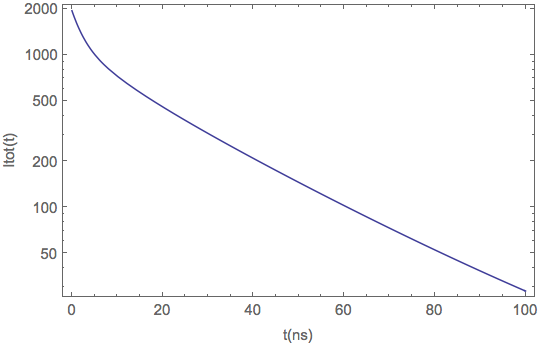
\includegraphics[scale=0.6]{../img/LXeScintillation2.png}
%	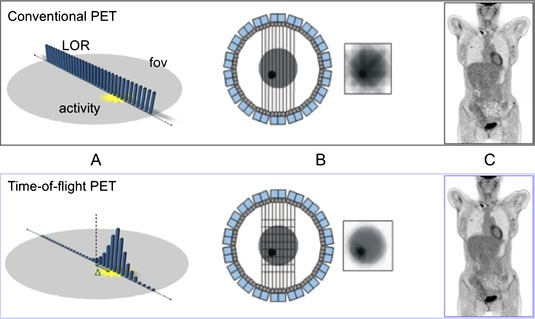
\includegraphics[width=.5\textwidth]{../img/TOFPET.jpg}
	\caption{\label{fig.scint} Intensity of scintillation in LXe. }
\end{figure}

Figure \ref{fig.scint} shows the total intensity of scintillation in LXe for a 511 keV gamma (resulting in a total of $N_\gamma =30000$~ VUV photons), adding the contribution of SE and SR processes. The resulting curve, which includes the contribution of SE and SR processes is well described in terms of the sum of two exponential distributions: 

\begin{equation}
I(t) = N_\gamma 0.07 \times \frac{e^{-t/\tau_1}}{\tau_1} + 0.93 \times \frac{e^{-t/\tau_2}}{\tau_2}
\label{eq.scint}
\end{equation}

Using equation \ref{eq.scint} it is possible to estimate the potential of LXe for TOF measurements, in particular compared with LYSO. The intrinsic CRT of a scintillator is proportional to the figure of merit 
$\psi = N_{pe}/\tau$, where $\tau$~is the lifetime of the scintillator and $N_{pe}$~is the number of photoelectrons, which in turn can be written as $N_{pe} = N_\gamma \times $PDE. Here $N_\gamma$ is the total number of photons emitted by the scintillator and PDE the overall particle detection efficiency of the sensor reading the scintillation light. 

Then, for LYSO: 

\begin{equation}
\psi = \frac{14000}{40} \times PDE = 350 \times PDE
\label{eq.lysoScint}
\end{equation}
%
while, for LXe:

\begin{eqnarray}
\psi_1 &=& \frac{30000 \times 0.07}{2.2} \times PDE = 954 \times PDE \\
\psi_2 &=& \frac{30000 \times 0.93}{27} \times PDE = 1033 \times PDE \\
\end{eqnarray}

Therefore:

\begin{equation}
\frac{\psi_{LXe}}{\psi_{LYSO}} = \frac{1987}{350} \sim 6 \times PDE
\label{eq.ratioScint}
\end{equation}

On the other hand, the scintillation light in LYSO is blue, peaking around 440 nm where the PDE of today's SiPMs reaches values as high as 50\%. Instead, the scintillation light of LXe peaks around 170 nm (VUV region). The NEXT experiment reads the LXe VUV scintillation light using conventional SiPMs coated with TPB \cite{Alvarez:2013gxa}. Alternatively, the MEG experiment will upgrade its LXe calorimeter using VUV-sensitive SiPMs \cite{Ogawa:2015ucj}.
\section{Monte Carlo study of the CRT in the LXSC2} The devices tested for the MEG upgrade have a PDE of about 15\%, and reaching a PDE of 20\% seems possible. In the case of SiPMs coated with TPB, the VUV light is absorbed by the wavelength shifter (with an efficiency of 80\%) and then re-emitted isotropically. Thus, the effective PDE is reduced to about 20\%. Thus:

 \begin{equation}
\frac{\psi_{LXe}}{\psi_{LYSO}} = \frac{1987}{350} \sim 3
\label{eq.ratioScint}
\end{equation}

In practice, the figure of merit is insufficient to estimate accurately the CRT resolution, since one has to add many other experimental effects. In the next section we address the most important ones through a detailed Monte Carlo study. 

\section{CRT in xenon: a Monte Carlo study}
\label{sec.CRT}

\begin{figure}[!bhtp]
	\centering
	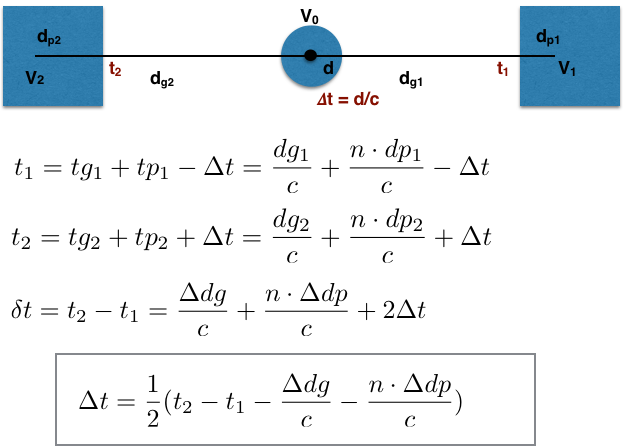
\includegraphics[scale=0.6]{../img/TOFSetup.png}
	\caption{\label{fig.scint} The setup simulated by this study. Back to back 511 keV gammas are emitted
	isotropically from $V_0$, and interact in two identical LXSC2, at vertices $V_1$~and
	$V_2$. The CRT ($\Delta t$), is found by subtracting the time of the first photoelectron recorded
	in each LXSC, $t_1$~and $t_2$~(or taking an average, see text for details) and correcting
	by the flight of time of the gammas ($\Delta d_g/c$) and the time of flight of the scintillation photons
	($n \cdot \Delta d_p/c$). }
\end{figure}  

In this section we present a Monte Carlo study quantifying the different factors entering the CRT for LXe. Figure \ref{fig.psetup} shows a scheme of  the LXe setup, simulated using the Geant-4 toolkit \cite{Agostinelli:2002hh} . Back to back 511 keV gammas are shot isotropically, from a common vertex $V_0$~ within the solid angle covered by two opposite LXSC2 ($5 \times 5 \times 5 {\rm cm^3}$) (in the LYSO the two LXSCs are replaced by LYSO crystals of $5 \times 5 \times 1.7 {\rm cm^3}$) . The gammas fly a distance $dg_1, dg_2$~before interacting in the LXSCs, at vertices $V_1, V_2$. Scintillation photons are produced according to equation \ref{eq.scint} for LXe (in the case of LYSO they are produced according to a single decay constant of 40 ns) and propagate through the LXe. Denoting $t_1,t_2$~to the time of the first photoelectron recorded in each one of the LXSC, The CRT can be written as:

\begin{equation}
\Delta t = \frac{1}{2}(t_2 - t_1 - \frac{\Delta d_g}{c} - \frac{n \cdot \Delta d_p}{c}) 
\label{eq.CRT}
\end{equation}
%
where $\Delta d_g/c$~is the time of flight difference from the emission to the interaction vertex of the two 511 keV gammas, and $n \cdot \Delta d_p/c$~is the time of flight difference from the interaction vertex to the
detection vertex (e.g, the position of the sensor) of the scintillation photons. 

Notice that, while the calculation of the term $\Delta d_g/c$~is immediate, finding the value
of $n \cdot \Delta d_p/c$~requires the knowledge of the refraction index of the medium (which in turn is a function of the wavelength of the scintillation photons) and the interaction vertices $V_1,V_2$, whose determination depends on the spatial resolution (and in particular of the DOI resolution) of the setup. Furthermore, the recorded time of the photoelectrons is affected by the time jitter of the sensor and the front-end electronics, as well as by the overall clock system. Other effects that affect the CRT are the existence of a rise constant for scintillation (absent in the case of LXe, but of te order of 70 ps for LYSO \cite{Seifert}), and the additional decay constant (about 1 ns) introduced if the SiPMs of the LXSC2 are coated with TPB to shift the VUV light to blue. 

In the remaining of this section we study systematically the various factors contributing to the CRT in LXe. 

\subsection*{Intrinsic CRT: effect of the DOI resolution}
We start our study by assuming that the scintillation in both LXe and LYSO is monochromatic and that the refraction indexes in both media are constant. We fix the scintillation of xenon to its peak (178 nm) and
the refraction index to 1.67. For LYSO we fix the scintillation at 430 nm and the refraction index to 1.82. 

\begin{figure}[!bhtp]
	\centering
	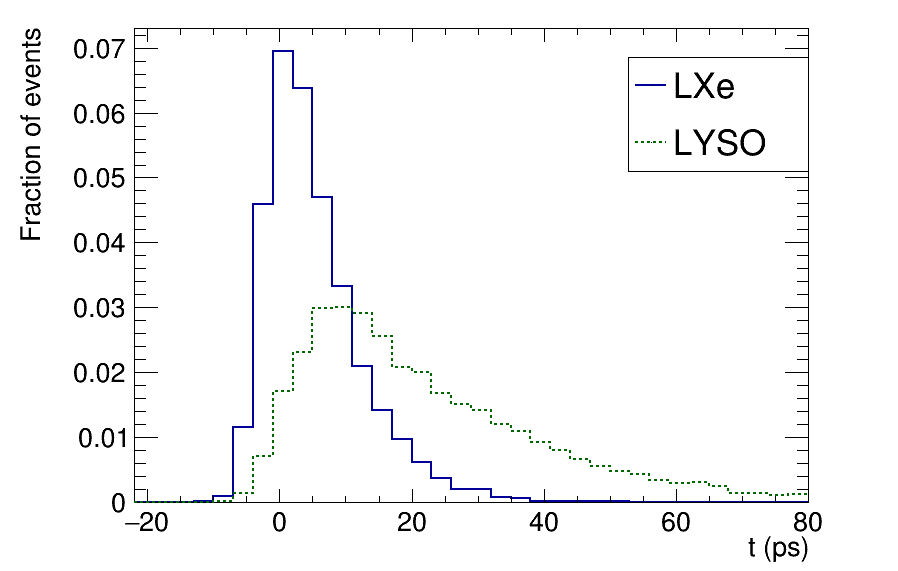
\includegraphics[scale=0.5]{../img/FirstPEScintLXeLYSO.png}
	\caption{\label{fig.firstPE} Arrival time of the first photoelectron in LXe (blue histogram) and LYSO (yellow histogram), after subtracting the time of flight of the incident gamma ($\Delta d_g/c$) and the time of flight of the scintillation photons ($n \cdot \Delta d_p/c$). }\label{fig.FirstPE}
\end{figure} 

Figure \ref{fig.FirstPE} shows the arrival time of the first photoelectron in LXe (blue histogram) and LYSO (yellow histogram), after subtracting the time of flight of the incident gamma ($\Delta d_g/c$) and the time of flight of the scintillation photons ($n \cdot \Delta d_p/c$). As expected, the VUV photons emitted by LXe arrive to the sensors earlier (and with a narrower distribution) than the blue photons emitted by LYSO. 

Notice that $\Delta d_p$~is the difference 
between the position of the interaction vertex and the position of the SiPM which records the photoelectron. 
The plot is computed introducing a resolution of 2 mm FWHM both in the transverse coordinates and
in the DOI (which corresponds to the resolution expected in the LXSC2). The jitter introduced by the DOI correction is:

\begin{equation}
\Delta t =\Delta z \times (n-1) \times 3.3\ \textrm{ps/mm}
\label{eq.DOI}
\end{equation}

For LXe, with n=1.67, $\Delta t = 4.4$~ps FWHM for a DOI resolution $\Delta z = 2$~mm FWHM. 
For LYSO, with n=1.82, $\Delta t = 5.4$~ps FWHM for a DOI resolution $\Delta z = 2$~mm FWHM. The effect is, therefore, small. Notice, on the other hand that a DOI resolution of 2 mm FWHM requires either a double layer of SiPMs (as in the LXSC2) or small monolithic crystals (for example, in Ref.~\cite{VanDamm2011} the authors find a DOI resolution varying between 1 and 4.5 mm FWHM for LYSO crystals of 
$20 \times 20 \times 12 ~{\rm mm^3})$). Instead, a conventional segmented LYSO crystal, 20 mm
thick would have a DOI r.m.s. resolution of 20 ${\rm mm}/\sqrt{12} = 5.8$~mm, thus 13 mm FWHM, resulting in a $\Delta t = 35.2$~ps FWHM.

\begin{figure}[!bhtp]
	\centering
	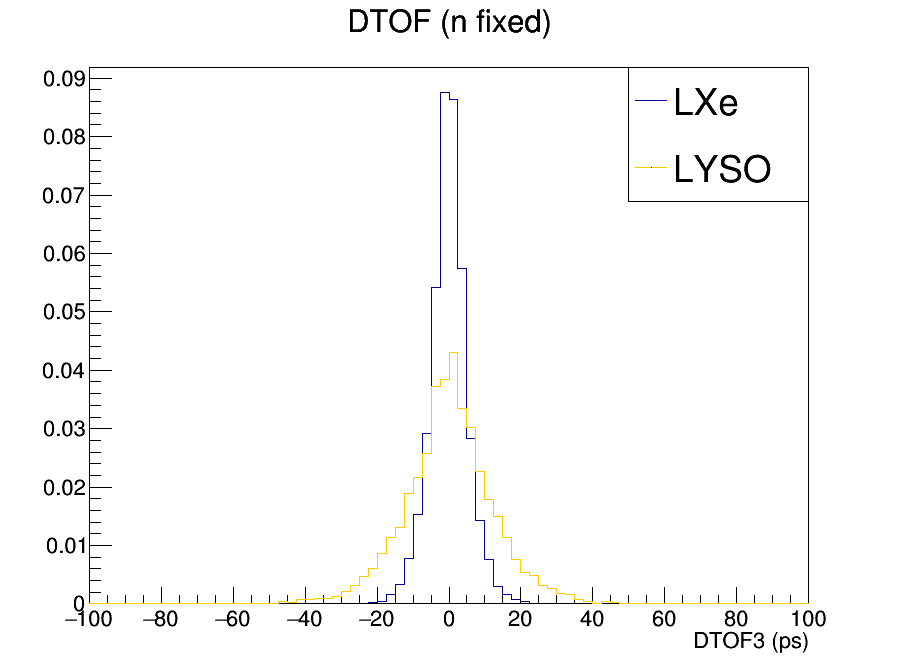
\includegraphics[scale=0.5]{../img/DTOFLXeLYSO.png}
	\caption{\label{fig.dtof} CRT (rms) in LXe (blue histogram) and LYSO (yellow histogram). The
	histograms are obtained introducing a spatial resolution of 2 mm for the transverse coordinates and
	the DOI, fixing the wavelength of the scintillation and the refraction index and setting the PDE of the SiPMs to one. }
\end{figure}

\begin{figure}[!bhtp]
	\centering
	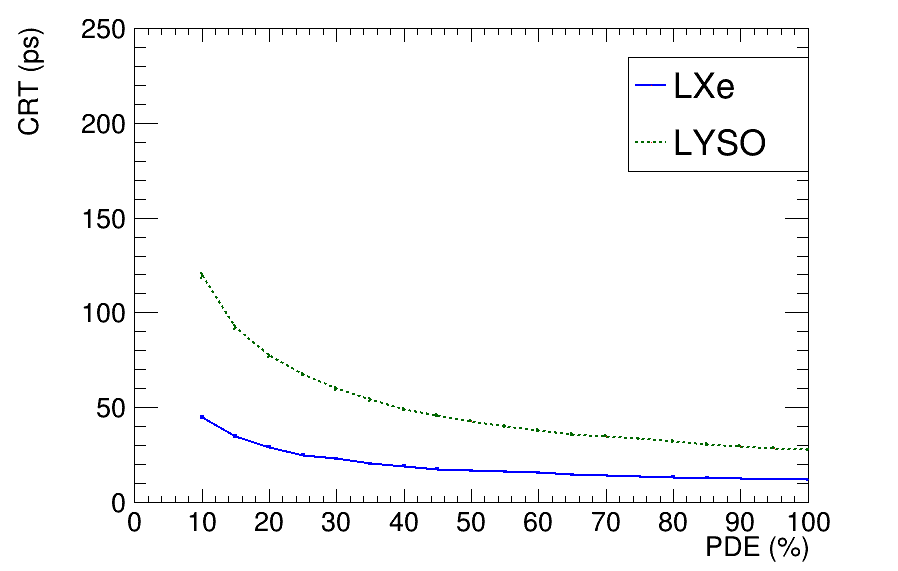
\includegraphics[scale=0.5]{../img/CRTvsPDELXeLYSONoJitterFstPE.png}
	\caption{\label{fig.crt1} CRT as a function of the PDE in LXe (red line) and LYSO (green line). }
\end{figure}

 Figure \ref{fig.FirstPE} shows the CRT (rms) for LXe (blue histogram) and LYSO (yellow histogram) for the ideal case of PDE = 1. The wider LYSO distribution is due to the slower decay constant. The intrinsic resolution of the LXSC2 setup (including the effect of the spatial resolution) is 5 ps (rms), while the
 intrinsic resolution of the LYSO setup is 12 ps (rms). Notice that, due to the contribution of the spatial resolution, the ratio of the CRT between LXe and LYSO is only about a factor 2, rather than a factor 6 suggested by the figure of merit. 
 
 Figure \ref{fig.crt1} shows the CRT as a function of the
 SiPM PDE. Notice that the dependence of the CRT with the PDE is flatter for LXe (red curve) than for LYSO (green curve), as expected given the fact that LXe is brighter scintillation than LYSO. On the other hand, the typical PDE of a blue sensitive SiPM (suitable for LYSO) is 50\% while the best VUV-sensitive SiPMs available today have a sensitivity of 15\% \cite{meg}. The value of the CRT for a PDE of 50\% in LYSO is $\sim$ 20 ps, while
the CRT for a PDE of 15\% in LXe is $\sim$ 15 ps.
  
\subsection*{Effect of the TPB decay constant}
%VUV sensitive SiPMs are currently still in the phase of development and are consequently very expensive (up to a factor 10) compared with blue sensitive SiPMs. 
% %We consider next the effect of coating the SiPMs of the LXSC2 with TPB. Notice that commercial VUV sensitive SiPMs are currently manufactured only by Hamamatsu\footnote{https://indico.hep.anl.gov/indico/getFile.py/access?contribId=157&sessionId=24&resId=0&materialId=slides&confId=625}, and suffer both from low PDE ($\sim 8\%$) and high cost (around 100 \euro\ per piece for 3 mm sensors, to be compared with 10-15 \euro\ for 3 mm conventional SiPMs). 
% Therefore VUV sensitive SiPMs are not a practical option
%for a PETALO scanner today, although the situation can improve considerably in the next few years given the interest in VUV sensitive sensors for the nEXO project \footnote{http://indico.inr.ru/event/4/session/1/contribution/8/material/slides/0.pdf} as well as for an upgrade of the 
%liquid xenon calorimeter of the MEG experiment \footnote{Eur.Phys.J. C73 (2013) no.4, 2365
%(2013-04-03)
%DOI: 10.1140/epjc/s10052-013-2365-2
%e-Print: arXiv:1303.2348}. 
%
%The baseline design of the LXSC2 proposes the use of conventional, blue-sensitive SiPMs coated with TPB, a technique that has been demonstrated by the NEXT experiment \cite{Alvarez:2012ub}. TPB coating introduces two effects in the response of a SiPM:
%
%\begin{enumerate}
%\item \item A reduction of the efficiency, associated with the absorption efficiency of the TPB at the LXe wavelengths ($\sim 80\%$) and the isotropic 
%re-emission of the blue photon (thus at most $\sim 50\%$~of the emitted photons enter the SiPM). 
% \item An effective delay of the first photoelectron due to the decay time of TPB ($\sim $ 1 ns). 
%\end{enumerate}

\begin{figure}[!bhtp]
	\centering
	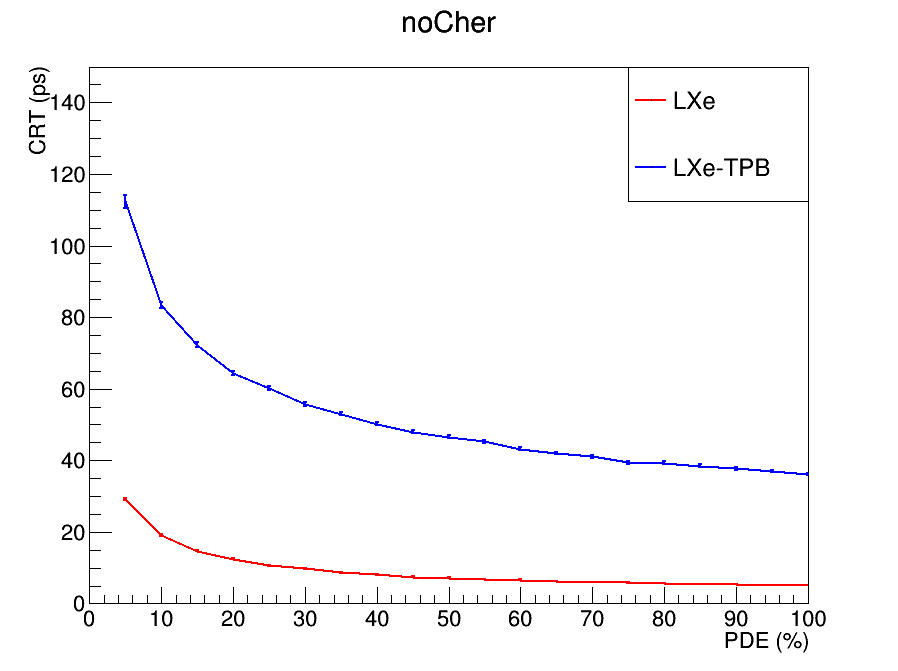
\includegraphics[scale=0.5]{../img/CRTvsPDELXeTPBNoJitter.png}
	\caption{\label{fig.crt2} CRT as a function of the PDE in LXe for VUV sensitive SiPMs (red line) and SiPMs coated with TPB (blue line). }
\end{figure}

Figure \ref{fig.crt2} shows the CRT as a function of the
 SiPM nominal PDE for VUV sensitive SiPMs (red curve) and TPB-coated SiPMs (blue curve) in LXe. Here we must compare the CRT achieved for VUV sensitive SiPMs with a PDE of 15\% ($\sim$ 15 ps rms) with the CRT achieved for blue sensitive SiPMs coated with TPB, taking as a reference a PDE of 50\% (this corresponds to the
 PDE for blue light,  however, the CRT is computed taking into account the effect of the TPB absorption and subsequent re-emission).  The CRT is this case is around 45 ps (rms). The degradation introduced by the TPB is, therefore quite large. However, as we will shortly see, the effect is
 considerably reduced when the impact of the jitter of the SiPM and front end electronics is included. 
  
\subsection*{Effect of the SiPM  and front-end electronics jitter}
  Next we introduce the effect of the jitter of the SiPM and front-end electronics, smearing the arrival time of the photoelectrons by a gaussian distributions with $\sigma = \sigma_{sipm} +  \sigma_{fee}$ and setting 
 $\sigma_{sipm} = 80$~ps, $\sigma_{fee} = 30$~ps. These values are typical of modern SiPMs and front-end electronics. 
 
 \begin{figure}[!bhtp]
	\centering
	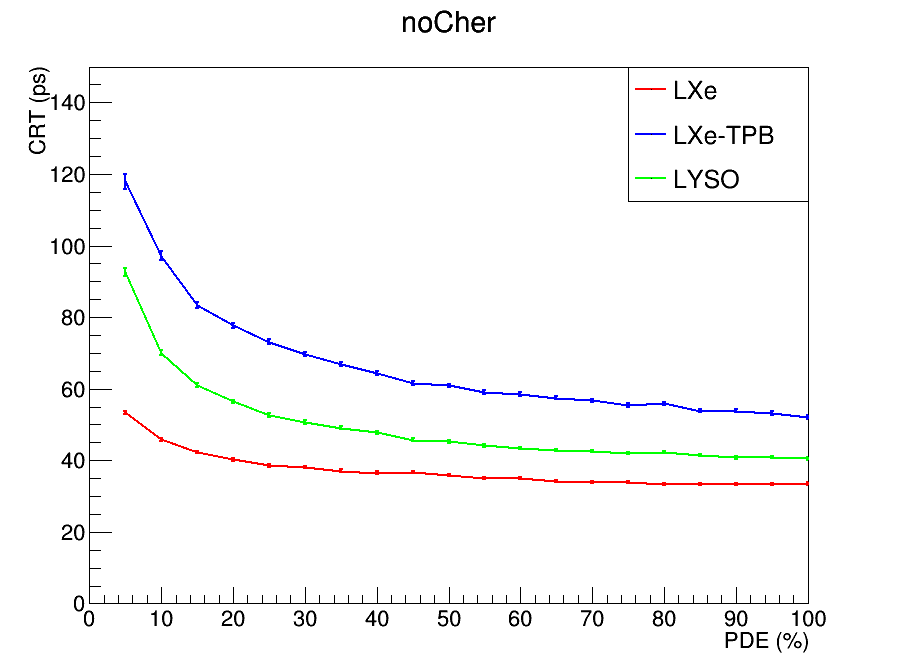
\includegraphics[scale=0.5]{../img/CTR_jitter_fixed_n.png}
	\caption{\label{fig.crt3} CRT as a function of the PDE in LXe for VUV sensitive SiPMs (red line) and SiPMs coated with TPB (blue line). The CTR for LYSO is also shown (green line). The CRT includes the
	effect of the jitter associated with the SiPM and the electronics and is computed using the first photoelectron.}
\end{figure}

Figure \ref{fig.crt3} shows the CRT as a function of the
 SiPM nominal PDE for VUV sensitive SiPMs (red curve) and TPB-coated SiPMs (blue curve) in LXe. The CRT for LYSO is also shown (green line). The CRT includes the
effect of the jitter associated with the SiPM and the electronics and is computed using the first photoelectron.
The CRT achieved for VUV sensitive SiPMs with a PDE of 15\% is $\sim$ 40 ps (rms), while with the CRT achieved for blue sensitive SiPMs with a PDE of 50\% and coated with TPB, is 60 ps (the CRT for LYSO and a PDE of 50\% is 50 ps, right in-between). The difference in CRT between the VUV sensitive case and the TPB coated case has been considerably reduced (from a factor 300 \% to a factor 50\%), since the jitter of the sensor and the electronics affects more the smaller CRTs. This finding points to the fact that the benefit of fast scintillators cannot be fully exploited unless the resolution introduced by the sensors and the electronics is reduced to values of the same order than the intrinsic CRT of the scintillator. 

\begin{figure}[!bhtp]
	\centering
	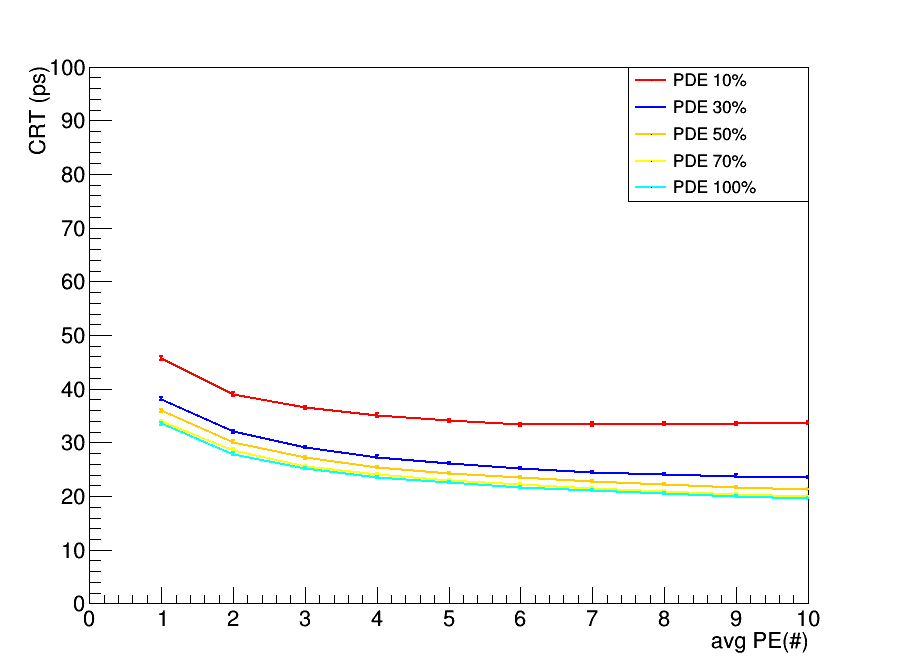
\includegraphics[scale=0.5]{../img/lxe_noCher_avg_npe.png}
	\caption{\label{fig.crt4} CRT as a function of the number of photoelectrons for several PDE in LXe for VUV sensitive SiPMs.}
\end{figure}

However, the CRT can be improved by using the first few photoelectrons recorded by the SiPM to compute an average. 
Figure \ref{fig.crt4} shows the CRT as a function of the number of photoelectrons for several PDE in LXe for VUV sensitive SiPMs. Using the first 10 photoelectrons, a CRT of 30 ps is achieved for a PDE of 15\%. 

\begin{figure}[!bhtp]
	\centering
	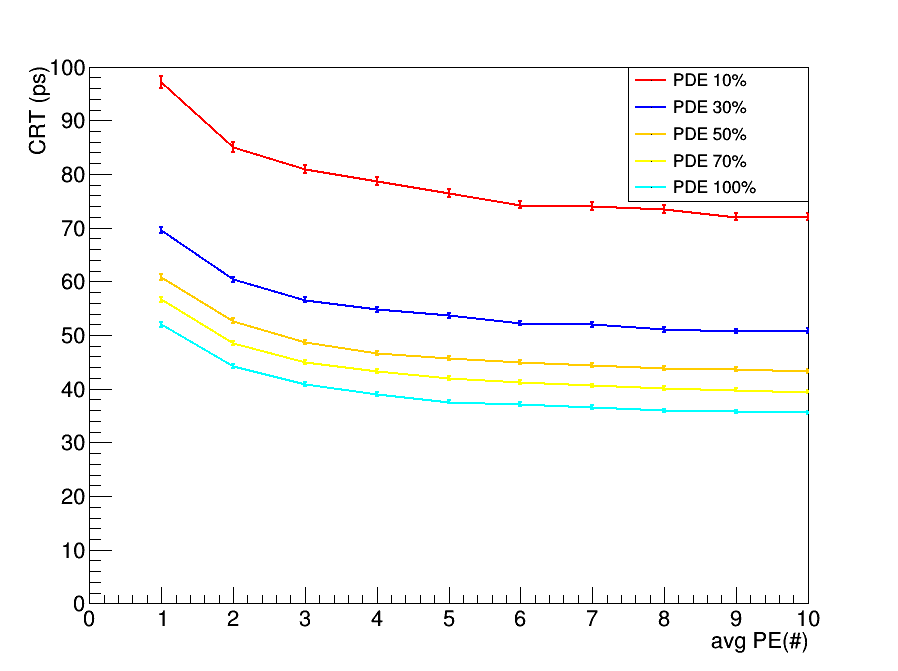
\includegraphics[scale=0.5]{../img/lxe_tpb_noCher_avg_npe.png}
	\caption{\label{fig.crt5} CRT as a function of the number of photoelectrons for several PDE in LXe for blue sensitive SiPMs coated with TPB.}
\end{figure}

Figure \ref{fig.crt5} shows the CRT as a function of the number of photoelectrons for several PDE in LXe for blue sensitive SiPMs coated with TPB. Using the first 10 photoelectrons, a CRT of 45 ps is achieved for a  PDE of 50\%. Notice that the use of the first few photoelectrons reduces the CRT of both VUV sensitive and blue sensitive SiPMs 
by a factor of 0.75 (improving fro 40 to 30 ps rms in the case of VUV sensitive devices and from 60 to 43 ps in the case of blue sensitive SiPMs coated with TPB).    

\subsection*{Including the effect of the variable refraction index}

\begin{figure}[!bhtp]
	\centering
	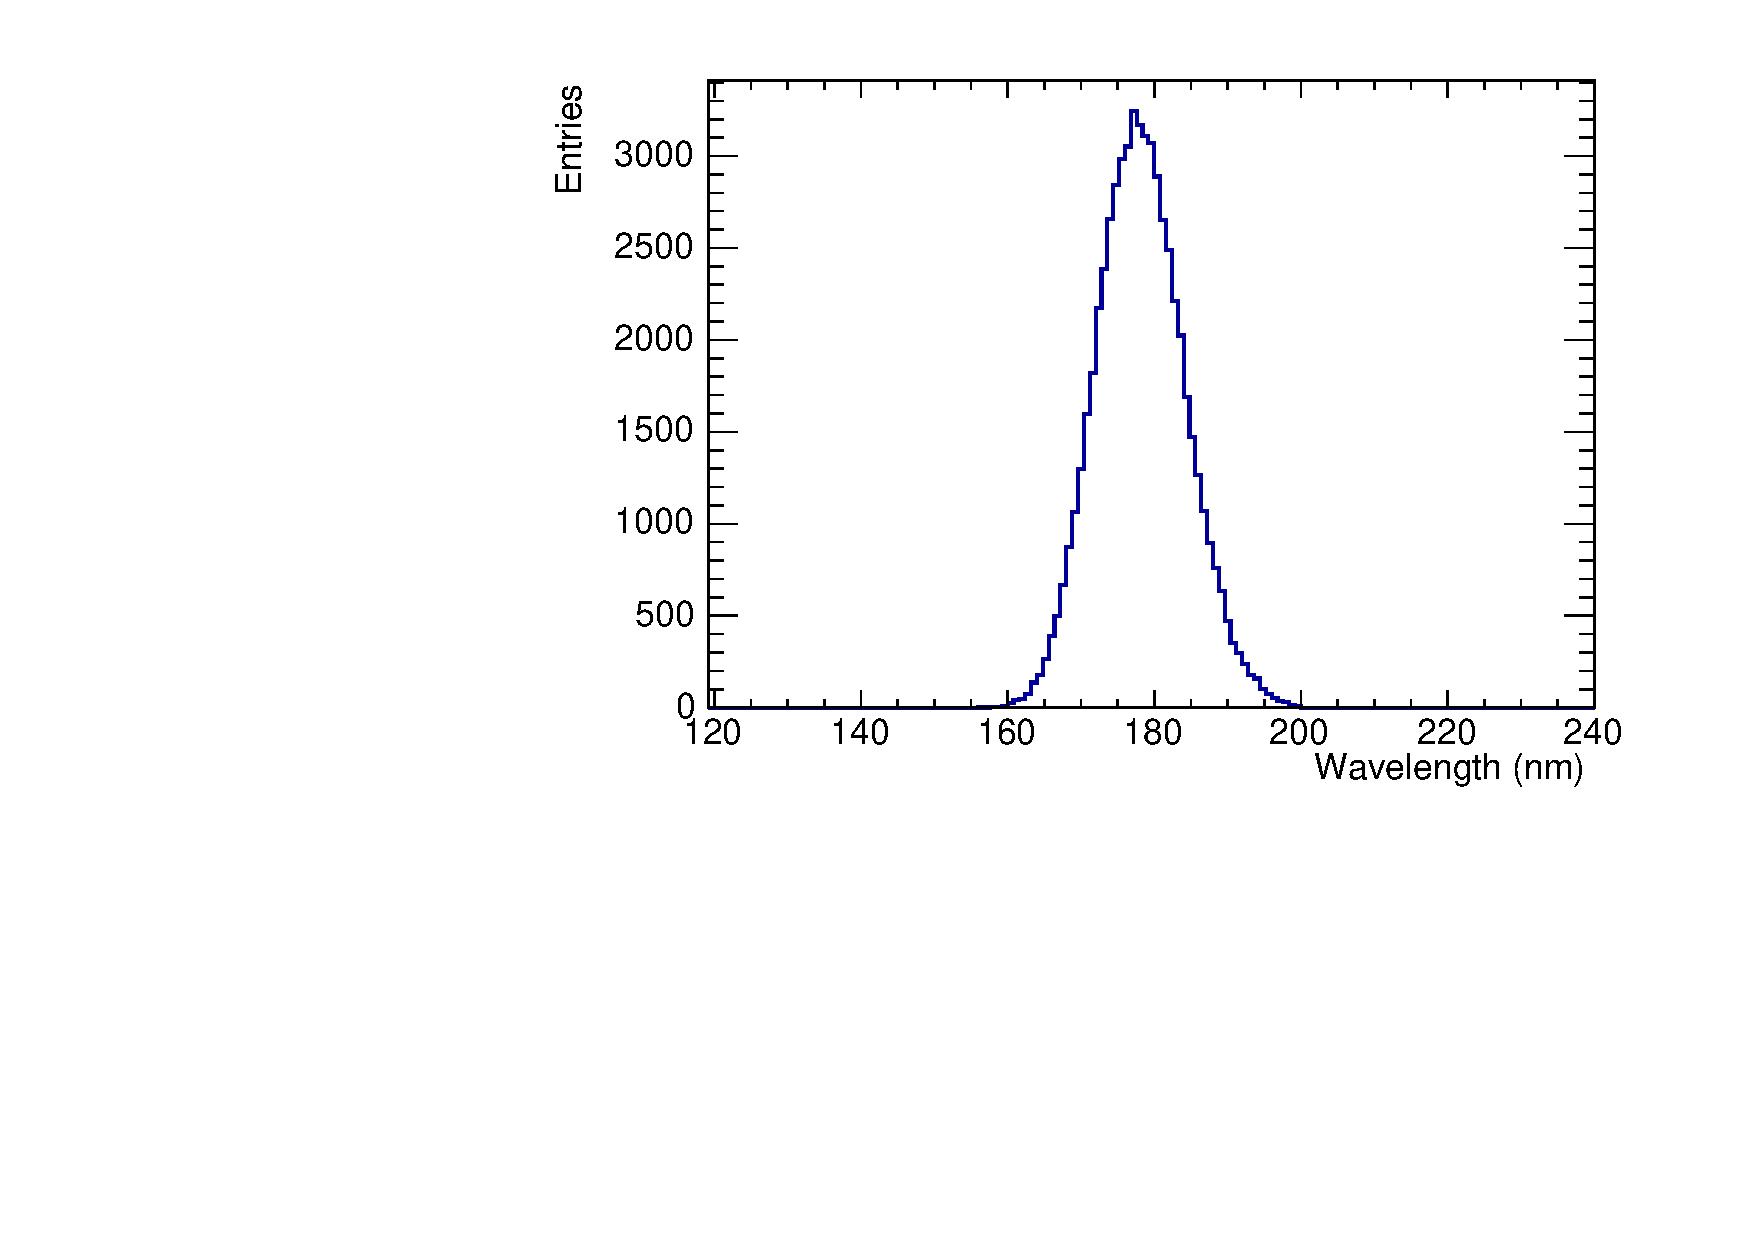
\includegraphics[scale=0.5]{../img/ScintillationSpectrumLXe.pdf}
	\caption{\label{fig.spectrumLXe} Distribution of the energy of scintillation photons in LXe.}
\end{figure}

\begin{figure}[!bhtp]
	\centering
	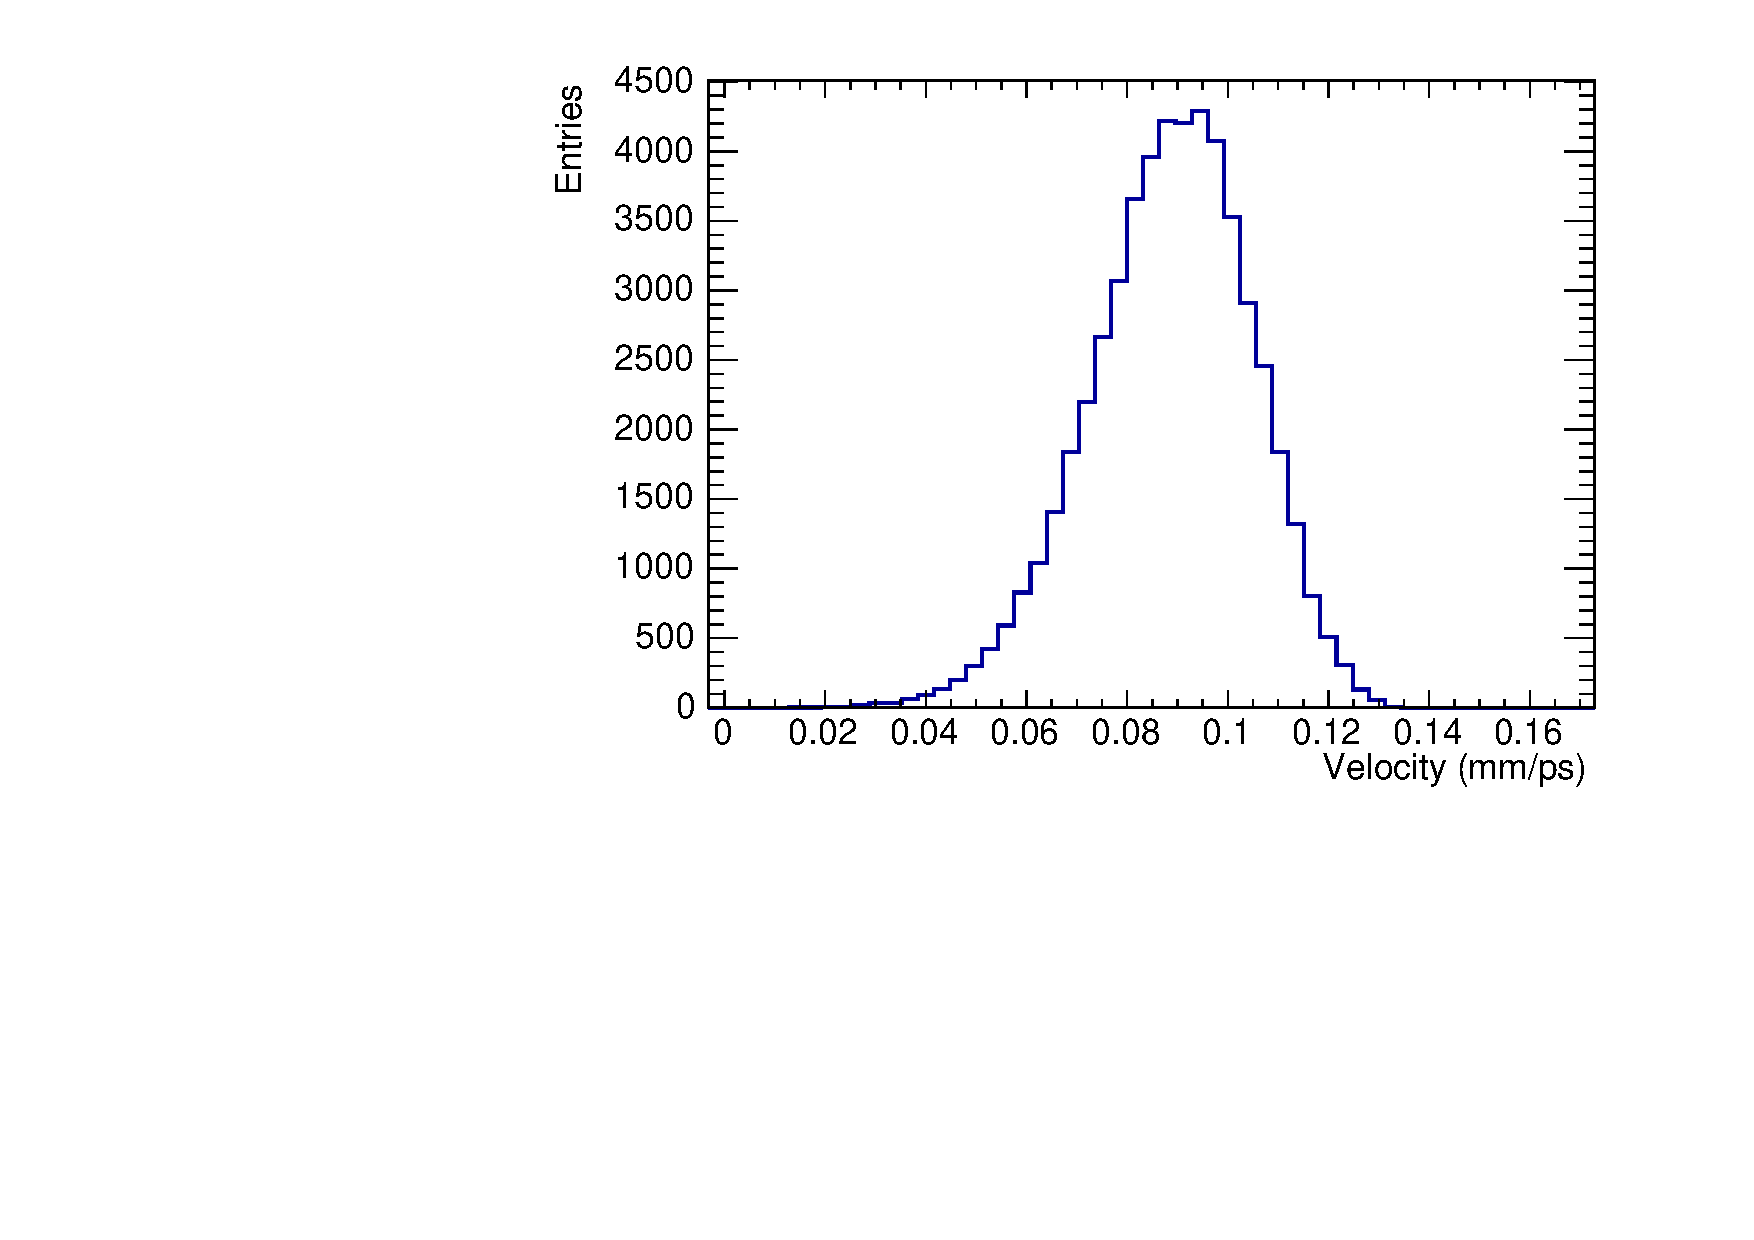
\includegraphics[scale=0.5]{../img/VelocityDistrLXe.pdf}
	\caption{\label{fig.vLXe} Distribution of the velocity of scintillation photons propagating in LXe.}
\end{figure}

\begin{figure}[!bhtp]
	\centering
	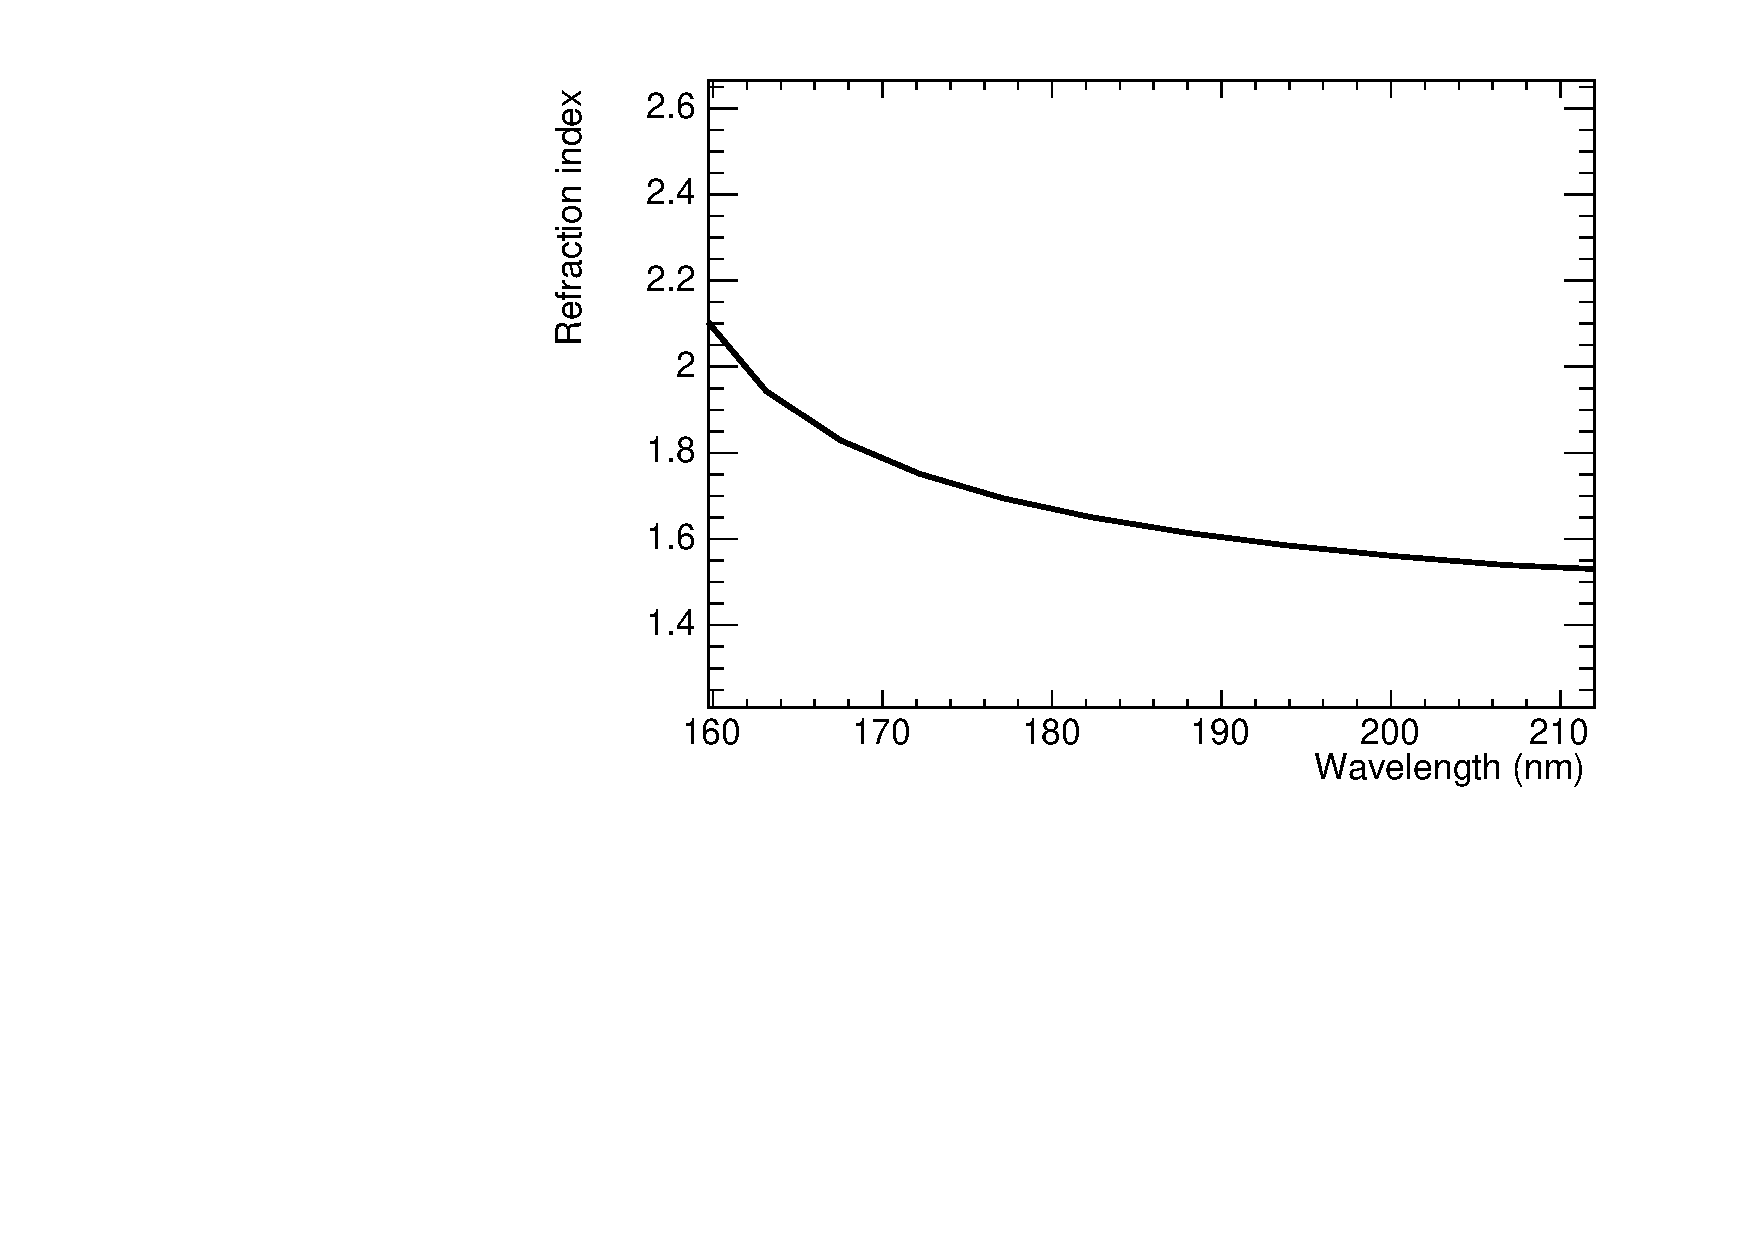
\includegraphics[scale=0.5]{../img/LXe_n_lambda.pdf}
	\caption{\label{fig.nlambda} LXe refraction index as a function of the wavelength of the optical photon.}
\end{figure}

  Next we introduce the fact that scintillation in LXe is not monochromatic but emitted with the spectrum shown in Figure \ref{fig.spectrumLXe}. On the other hand, the refraction index in xenon is a function of the wavelength, as shown in Figure \ref{fig.nlambda}. This implies that the VUV photons propagate with different velocities depending of their wavelength, as shown in Figure \ref{fig.vLXe}. To take into account this effect, one must use the average group velocity of the photons instead of the constant term $n/c$
in equation \ref{eq.CRT}. This introduces an extra smearing, due to the spread of the average velocity. The effect worsens slightly the CRT of the VUV sensitive SiPMs, resulting in a value of about 35 ps rms for a PDE of 15 \%, but is negligible in the case of TPB coated SiPMs where the CRT is still 43 ps for a PDE of 50\%. The corresponding value for LYSO and 50\% PDE is similar ($\sim$ 42 ps rms). 
  
  \subsection*{Including the effect of the overall syncronization}
  Finally, we have included the effect of the overall syncronization of a large system, introducing a binning of 25 ps in the recording of the photoelectrons (this corresponds to the binning offered by a number of TOF ASIC\footnote{PETSYS}). The effect turns out to be negligible.  
  
\subsection*{CRT of a PETALO-LXSC2 scanner}
In summary, we find that the CRT of a PETALO-LXSC2 scanner can be as good as 35 ps rms or 80 ps FWHM if VUV sensitive SiPMs with a PDE of 15\% are used. This value seems to be within reach of the current technology, although high cost is still an issue for this type of devices. For reference, a PDE of 30\% would result in a CRT of 20 ps rms or 46 ps FWHM. 

On the other hand, it appears feasible to build a large PETALO scanner using large (6 mm) and comparatively cheap SiPMs sensitive to blue light coated with TPB. For a typical PDE of 50\% we find a CRT of
43 ps rms or $\sim$100 ps FWHM. A similar value is found for the LYSO reference setup.


\section{Summary and outlook}\label{sec.conclu}

We have studied the CRT that can be obtained by a PETALO scanner based in the LXSC2 cell. The intrinsic resolution of the cell (corresponding to an ideal VUV sensitive sensor of PDE one) is 5 ps rms (11.5 ps FWHM), of which DOI uncertainty contributes with about 5 ps. Introducing a realistic PDE of 15\%, corresponding to the best currently achieved by VUV-sensitive SiPMs, still results in an excellent CRT of  15 ps rms (35 ps FWHM). Alas, this impressive performance is partially washed away by the effect of the SiPM jitter (80 ps rms) and front end electronics (30 ps rms). Averaging the CRT over the first 10 photoelectrons, a CRT of 30 ps rms (69 ps FWHM) is found. Finally, introducing the dependence of the 
refraction index of xenon with the photon wavelength (as well as a time binning of 25 ps reflecting the overal clock) one finds a CRT of 35 ps rms or 80 ps FWHM. It follows that a PETALO scanner based in the LXSC2 cell equipped with VUV sensitive SiPMs of relatively large PDE (15\% or better) could reduce the CRT of a large system below the 100 ps threshold. 

On the other hand, we find that using blue sensitive SiPMs coated with TPB results in a CRT of about 100 ps FWHM for a PDE of 50\%. This is still an very good result, in particular given the competitive cost of today's SiPMs and  front-end electronics.  In summary, it appears feasible to build a PETALO scanner with existing technology, combining the advantages of large sensitivity (due to increased large axial acceptance afforded by the low cost of xenon compared with LYSO), good energy and spatial resolution, and excellent CRT.     

\section*{}

\bibliography{biblio.bib}

\end{document}